\section{\translate{Implementation}/\translate{Design}}\label{sec:implementation} 
Choose only one of the headlines. In this chapter you will explain all the technical details of your
work. Start this chapter with an overview of your work and an overview block figure with the
protocols, algorithms, and technologies written out. Basically, as form of UML component diagram.
You can also use storyboards, mock-up designs, state diagrams to show the overall structure. See
Figure 1 for an example. All figures must be references from the text. 
\cref{fig:overview}. All figures must be references from the text.

\begin{figure}
  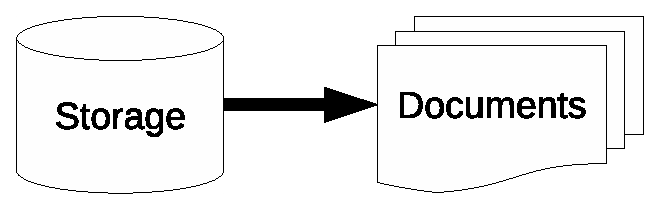
\includegraphics[width=5cm]{Figures/Latex_figure1.eps}
  \caption{System overview}\label{fig:overview}
\end{figure}

\subsection{First part of the overview figure}\label{subsec:overview1}
Use a top-down approach, divide and conquer, split the figure into relevant pieces. Explain each
piece in detail, use titles that can be found in the overview figure. Use flow charts, UML diagram,
pseudocode etc.\ but no real code. Refer to the appendix for the actual source code.

\subsection{Another part of the overview figure}\label{subsec:overview2}
Another piece of the solution.

\subsection{Etc.\ until all parts are covered from the overview figure}
Another piece of the solution. Etc.\

\subsection{\translate{Measurement}/
            \translate{Evaluation setup}}\label{subsec:eval_setup} 

Remember to explain how you will measure/evaluate your implementation and how your test bench has
been built/setup/implemented.
